\section{Protein synthesis}

Lastly, we turn our attention to the process of translation. So far in our
various estimates there has been little to suggest any apparent limit to how
fast a bacterium might divide under steady-state growth. Even in our examples of
\textit{E. coli} grown rapidly under different carbohydrate sources
(\FIG{carbon_tport}(B)),  cells are able to utilize less preferred carbon
sources by inducing the expression of additional membrane transporters and
enzymes. [Maybe go into Hwa style resource allocation with references added]. In
this respect, gross overexpression of a protein can lead to a reduction of the
growth rate.

We can determine the translation-limited growth rate by noting that the total
number of peptide bonds created as the cell doubles $N_{aa}$ will be given by,
$\tau \cdot r_t \cdot R$. Here, $\tau$ refers to the doubling time of the cell
under steady-state growth, $r_t$ is the maximum translation rate, and $R$ is the
average number of ribosomes in the cell. With the growth rate related to the
cell doubling time by $\lambda = ln(2)/\tau$, we can write the
translation-limited growth rate as,

\begin{equation}
\lambda_{\textrm{translation-limited}} = \frac{ln(2) \cdot r_t \cdot R}{N_{aa}}.
\end{equation}
Alternatively, since $N_{aa}$ is related to the total protein mass through the
molecular weight of each protein, we can also consider the growth rate in terms
of ribosomal mass fraction. This calculation in shown in \FIG{translation_1}(A).
This allows us to rewrite the growth rate as,

% By approximating the average molecular weight of an
% amino acid as 110 Da, the cellular protein mass $M$ can be estimated $N_{aa}
% \cdot 110 Da / N_A$, where $N_A$ is Avogadro's number. The total mass associated
% with $R$ ribosomes will be given by $m_R$ = $(L_R * 110 Da) * R / N_A$,  where
% the $L_R$ is the total length in amino acids that make up a ribosome,  and $L_R
% * 110 Da$ is the approximate molecular weight of the entire ribosomal complex. In terms of
% cellular mass $m$ and ribosomal mass $m_R$, we can then write the growth rate as,
%
% \begin{equation}
% \lambda_{max} \approx \frac{ln(2) \cdot r_t \cdot m_R/(L_R * 110 Da) }{(m_{protein}/110 Da)}.
% \end{equation}
% Denoting the ribosomal mass fraction
% by $\Phi_R$, which is just the ratio of ribosomal mass divided by the total cellular mass,
% $M_R/M$, we find that the translation-limited growth rate is given by,

\begin{equation}
\lambda_{\textrm{translation-limited}} \approx \frac{ln(2) \cdot r_t}{L_R}  \Phi_R,
\label{eq:translation_limit_growth_rate}
\end{equation}
where $L_R$ is the total length in amino acids that make up a ribosome, and
$\Phi_R$ is the ribosomal mass fraction. This is plotted as a function of
ribosomal fraction $\Phi_R$ in \FIG{translation_1}(A), with a translation rate
$r_t = 17 aa/s$ and $L_R = $[] $aa$, which corresponds to the length in amino
acids for all ribosomal subunits of the 50S and 30S complexes and elongation
factor required for translation.

Perhaps the first thing to notice is that there is a maximum growth rate at
about $\lambda \approx 6 hr^{-1}$, or doubling time of
about 7 minutes. This maximum growth rate can be viewed as an inherent speed
limit due to the need for the cell to double the cell's entire ribosomal mass.
Interestingly, this limit is independent of the absolute number of ribosomes,
but rather  is simply given by time to translate an entire ribosome, $L_R/ r_t$.
As shown in \FIG{translation_1}(B),  we can reconcile this with the observation
that in order  to double the average number of ribosomes, each ribosome must
produce a second  ribosome. This is a process that cannot be parallelized
further.

% Here we have implicitly assumed that translation proceeds randomly, without
% any apparent  preference between ribosomal or non-ribosomal mRNA, which
% appears reasonable.
% [NB:I wonder if there is something to be said about having to add X rRNA for each ribosome]


Since a cell consists of more than just ribosomes, we can see that for $\Phi_R$
in the range of about 0.1 - 0.3, the maximum growth rate is in line with
experimentally reported growth rates around 0.5 - 2 $hr^{-1}$. Here we have
implicitly assumed that translation proceeds randomly, without preference
between ribosomal or non-ribosomal mRNA, which appears reasonable. Importantly,
in order for a cell to scale this limit set by $\Phi_R$ the cell must increase
it's ribosomal abundance, either by synthesizing more ribosomes or reducing the
fraction of non-ribosomal proteins.

\begin{figure}
  \begin{fullwidth}
        \centering{
            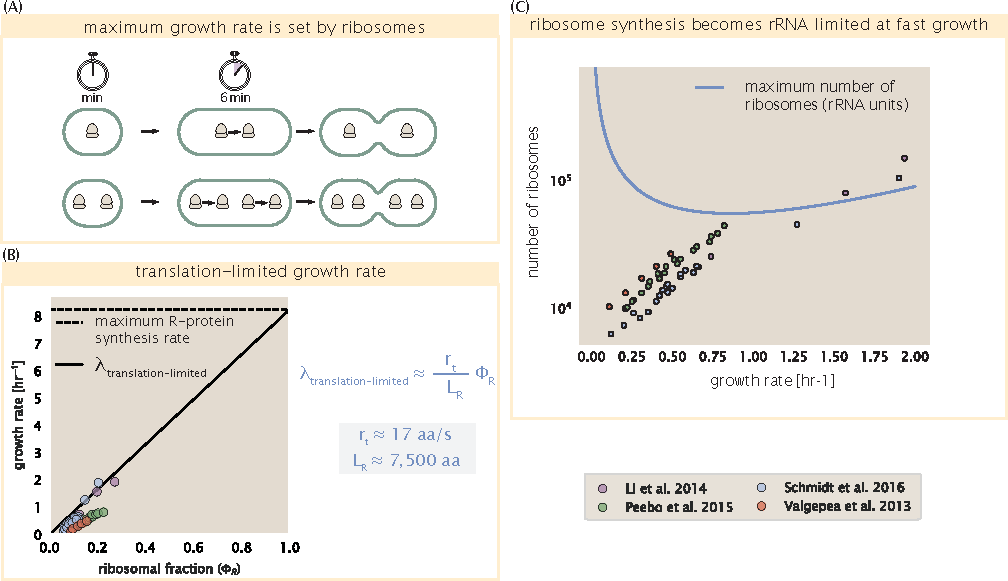
\includegraphics{main_figs/fig7_ribosome_growth_limit_2.pdf}
            \caption{\textbf{Translation-limited growth rate.} (A) Here we consider
            the translation-limited growth as a function of ribosomal fraction. By
            mass balance, the time required to double the entire proteome ($N_{aa}$ /$r_t \cdot $) sets the translation-limited growth rate, $\lambda_{\textrm{translation-limited}}$. Here $N_{aa}$ is effectively the number of peptide bonds that must be translated, $r_t$ is the translation elongation rate, and $R$ is the number of ribosomes. This can also be re-written in terms of the ribosomal mass fraction $\Phi_R = m_R$ / $m_{\textrm{protein}}$, where $m_R$ is the total ribosomal mass and $m_{\textrm{protein}}$ is the mass of all proteins in the cell. $L_R$ refers to the summed length of the ribosome in amino acids. $\lambda_{\textrm{translation-limited}}$ is ploted as a function of $\Phi_R$ (solid line). (B) The dashed line in part (A) identifies a maximum growth rate that is set by the ribosome. Specifically, this growth rate corresponds to the time required to  translation an entire ribosome, $L_R/ r_t$
            . This is a result that is independent of the number of ribosomes in the cell as shown schematically here. (C)}
        \label{fig:translation_1}
        }
  \end{fullwidth}
\end{figure}


One additional point to note is that across
different species of bacteria, cells do not decrease their
ribosomal abundance to zero in the limit of poorer nutrient condition [CITE?]. Indeed,
some organisms appear to have constant ribosomal abundance irrespective of their
growth rate [NB: ask Griffin and figure out what organism this is]. From the
perspective of a bacterium dealing with uncertain nutrient conditions, there is
likely a benefit for the cell to maintain some relative fraction of ribosomes to
support rapid growth as nutrient conditions improve. In addition, given their
massive size at about 850 kDa, they may play an as-yet fully understood role as
a crowding agent in cellular function \cite{delarue2018, solerbistue2020}. If we
consider a scenario where nutrient conditions become poorer and poorer, there
must be a regime where the cell has more ribosomes than it can utilize. While
this perhaps suggests less import to the  process of translation, it is
important to recognize that in order for a cell to maintain steady-state growth,
the cell's translation capacity must be mitigated. Otherwise, ribosomes will
deplete their supply of amino acids and this will bring translation and cell
growth to a halt (\FIG{translation_1}(C)). We will consider the consequences of
this in the case of \textit{E. coli} next.

% [NB: should I try to show this more quantitatively here?? Perhaps we can dig into
% details in E coli specific section.]

\subsection{Multiple replication forks provide one strategy to support faster growth.}

% [NB: need to think about rRNA copy number and what this might mean]
% [NB: another point that might be worth noting is that ribosomal genes are among the
% most highlight produced - so it's not a simple matter of 'inducing' expression to
% make more.]

We now turn to our proteomic data from \textit{E. coli} and plot the ribosomal
fraction as a function of reported growth rate. Here we find that the ribosomal
fraction always increases with growth rate. This is consistent with the behavior
expected for \textit{E. coli}, and an observation of intense study related to
the so-called nutrient-limited growth law. In terms of absolute ribosomal
abundance, we find that cells increase both their quantity and cellular
concentration at faster growth.

One feature of \textit{E. coli}, as well as other bacteria like \textit{B.
subtilis}, is the ability to begin replication of multiple copies of its genome
during a single cell cycle. This is achieved through multiple initiation forks
and nested DNA replication. [need to refer to work from to Jun lab here!! -
under adder mechanism, the cell appears to add a certain cell mass in proportion
to its number of origins]. We find that the ribosome copy number increases in
proportion to the expected number of origins. The process of nested DNA
replication will lead to a bias in gene dosage for genes closer to the origin of
replication \cite[], Importantly, ribosomal protein and rRNA genes are closer to
the origin of replication \cite{scholz2019} and this provides a natural way for
\textit{E. coli} to bias the proportion of ribosomes at faster growth without
the advent of additional gene regulation strategies. Given that ribosomal genes
in \textit{E. coli} appear to be transcribed at their maximal rate at fast
growth rates [cite??],  increasing ribosomal copy number through increased gene
dosage represents a creative  approach for the cell to grow faster without gross
down-regulation of non-ribosomal genes.

% Next consider growth below the capacity of ribosomes.


% Maybe start with E. coli section by noting details from Jun lab as a given. Si et al 2017: The average cell size increased exponentially with respect to the nutrient-imposed growth rate l ( = ln2/t), in agreement with the nutrient growth law [1] (Figure 1; see the Supplemental Information). The ribosome fraction 4R increased linearly with the growth rate, confirming previous re- ports [8, 9]. tC and tcyc were both constant for a wide range of growth conditions at tC = 38.00 ± 4.50 and tcyc = 75.10 ± 7.20 (Fig- ure 1C; see the Supplemental Information) [21, 22].
%  AND it follows 'adder' model of cell division

%  Noting Fig7A, highlight that for cells to optimize their growth , they will benefit by varying their ribosomal abundance; and that they can do this by varying gene dosage - since otherwise it is not obvious how they might make more ribsoomes.

% ****** Data from that 2020 paper on ppGpp and Si et al, and Zhu et al. all point to an increase in ribosomal content with higher number of origins (t_cyc/ tau)
% ->> Can I show this somehow , maybe an important point.



% Might be worth noting that E. coli doesn't grow if you knockout regulation by ppGpp. FROM Zhu et al. 2019 NAR: On the other hand, low ppGpp levels seem to be adverse for biomass growth as well, as shown by the inability of ppGpp- null strain to grow in minimal medium (21,32,33), suggest- ing the importance of maintain an optimal ppGpp level for cell growth.

% It'll remain to be determined whether perturbations like those in Dai et al.,
% and the more recent paper in NAR is consistent with a varying number of
% origins. But I think it's curious that they see a trend exactly like the trend
% in nutrient-limited growth when they vary ppGpp, and roughly similar (high)
% active fraction of ribosomes. I guess is that this type of regulation works
% on more than just ribosomes, and perhaps it is changing number of origins.
% Another point is that fraction of ribosomes again seems to move toward
% a non-zero limit, which bodes well with number of ribosomes depending on
% number of DNA ori.

% I don't think it's trivial to 'up' regulate ribosomal synthensis. This seems like an importsnt consideration.

% I think it might be worth noting that we can think of this changing gene dosage as also changing the genome makeup of the cell.



\begin{figure*}
    \begin{fullwidth}
    \centering{
        \includegraphics{main_figs/fig8_ribosome_growth_limit_ecoli_.pdf}
        \caption{\textbf{.} (A) (B) (C).}
        \label{fig:translation_2}
    }
    \end{fullwidth}
\end{figure*}
